To isolate the different parts of the system and limit overlap between groups, the project was divided in accordance with figure~\ref{fig:architecture} into three parts, frontend, backend and tester.

Frontend was designed to avoid keeping state. By doing so, the user-facing components could scale out to multiple backend servers and keep commonly used content cached. This would allow for better load-balancing where frontends could be geographically distributed and yield lower latencies.

Backend was designed to control the database and to keep a centralized management of state transitions. A feature that was discussed, but not investigated, was to shard the data between backends. That would have allowed even greater flexibility in the development of the platform, should it be used in more than one place.

Since tester could be used by other projects than the Gamified Programming Platform, it was designed to be idempotent and stand-alone. This meant that any tester server would yield the same result every time it was queried and have no prior knowledge of the system.
\begin{figure}
    \centering
    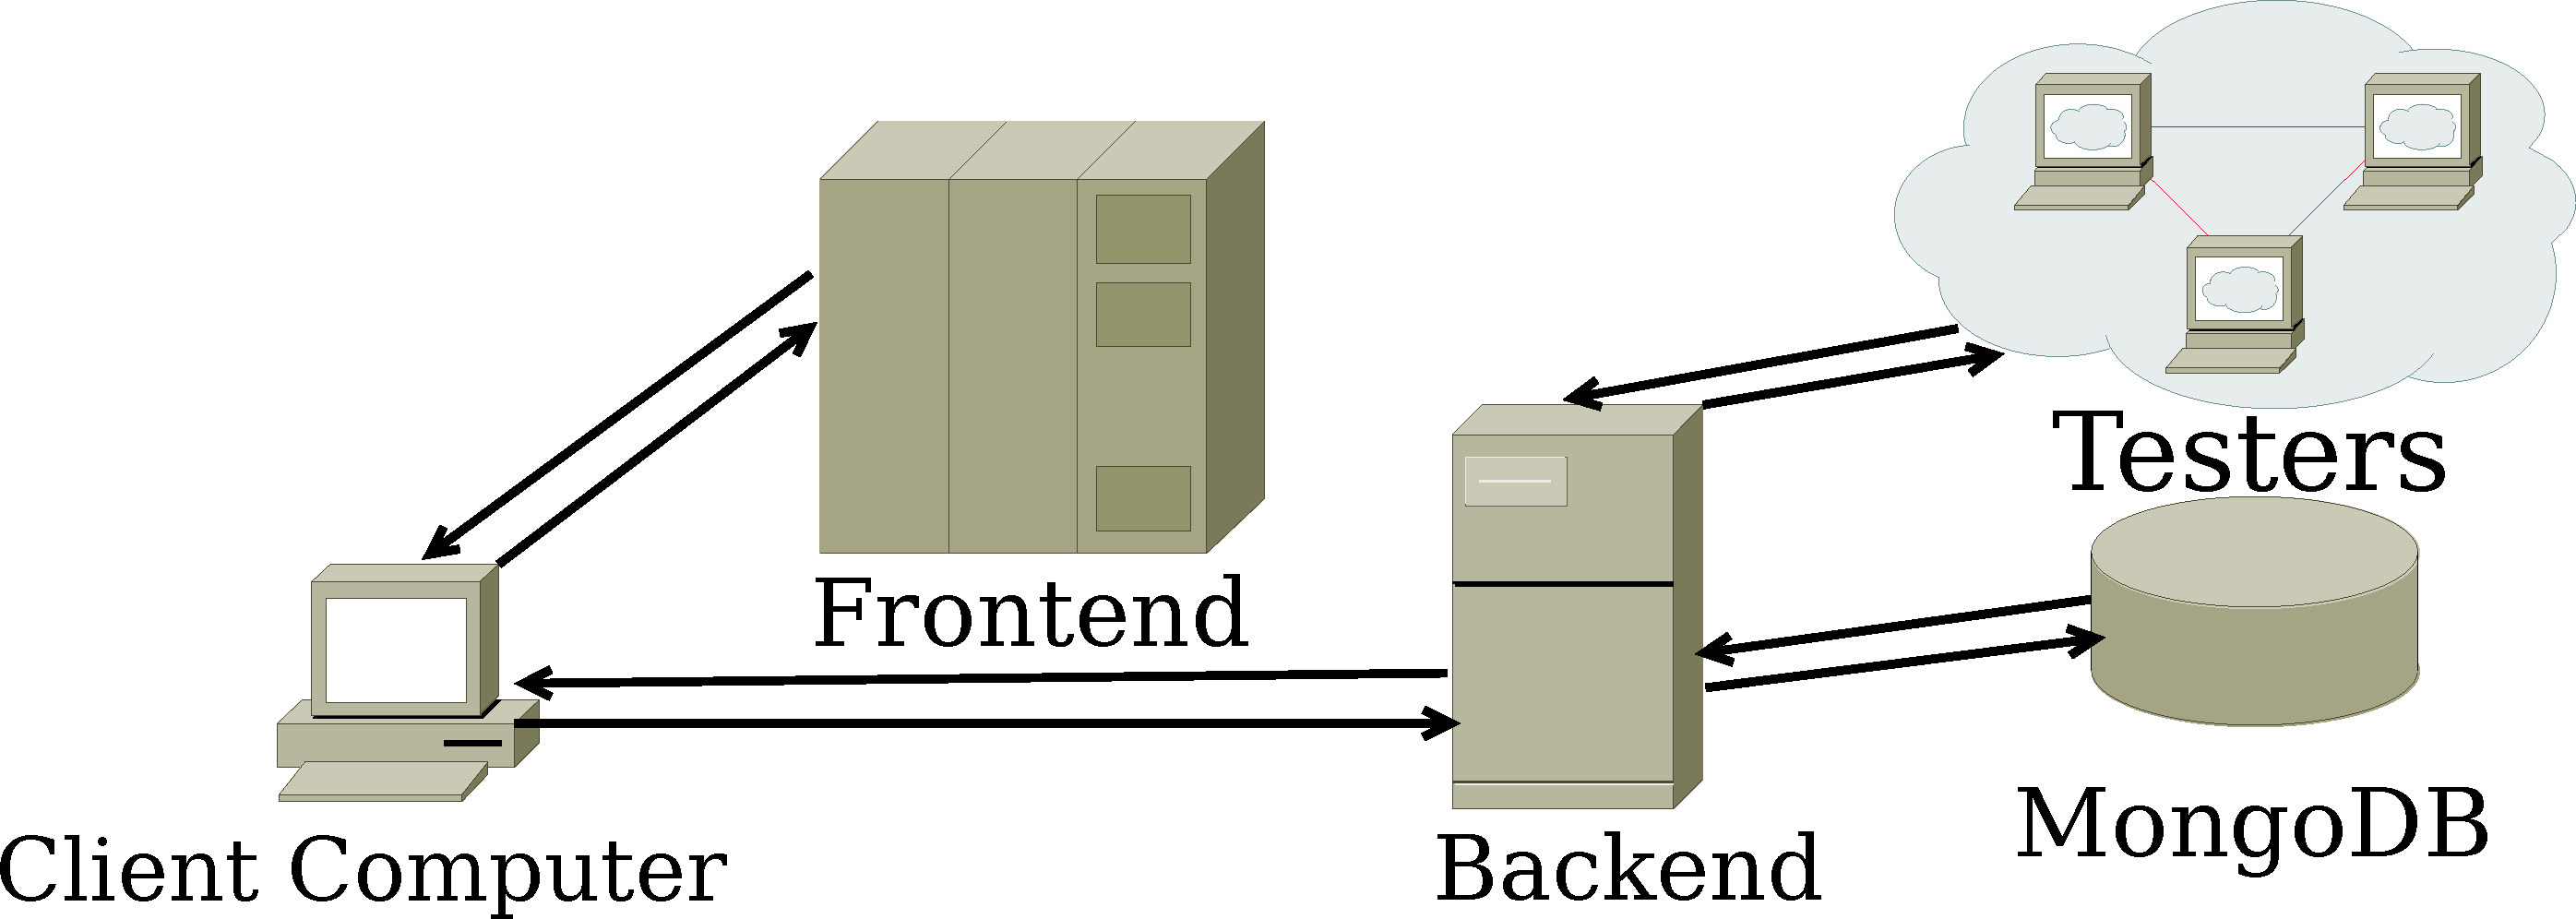
\includegraphics[width=.9\textwidth]{img/architecture.pdf}
    \caption{An overview of the architecture: First, some client interacts with the frontend, which uses javascript to send requests for resources on the backend. Then, the backend communicates with its database to serve resources. When the backend receives a request for testing, it retrieves assignment information, couples it with input data and sends it to the testers, which respond with the result of the test back through the request chain.}\label{fig:architecture}
\end{figure}
